\documentclass[a4paper]{article}

\usepackage[utf8]{inputenc}
\usepackage[portuges]{babel}
\usepackage{a4wide}
\usepackage[pdftex]{hyperref}
\usepackage[T1]{fontenc}
\usepackage{graphicx}
\usepackage{fancyvrb}
\usepackage{indentfirst}
\usepackage{array}
\usepackage{float}

\title{Projeto de Laboratórios de Informática 1\\Grupo g166}
\author{Mariana Miranda (a77782) \and Helena Poleri (a78633)}

\begin{document}

\maketitle
\begin{abstract}
Para esta segunda fase do projeto de Laboratórios de Informática 1 (LI1), foi nos pedido que realizássemos três tarefas relacionadas com o \emph{puzzle} Sokoban, exceto a segunda. Foi também a primeira vez que trabalhámos com a biblioteca gráfica \emph{Gloss}, que utilizámos para as últimas duas tarefas, das quais uma consistia no desenvolvimento da \emph{interface gráfica} do jogo \emph{Sokoban}.

Conseguimos atingir os nossos objetivos ao finalizar as três tarefas. As duas que eram objeto de avaliação do \emph{Mooshak}, foram totalmente aceites por este. Para além disso, e como a última tarefa de criação da interface gráfica era aberta, ainda conseguimos adicionar os extras que queríamos ao jogo.
\end{abstract}
\newpage

\tableofcontents
\listoffigures
\listoftables

\newpage
\section{Introdução}
\label{sec:intro}

Desenvolvida no âmbito da disciplina de Laboratórios de Informática 1 (LI1), da Licenciatura em Engenharia Informática da Universidade do Minho, esta segunda fase do projecto, desenvolvida na linguagem de programação funcional \emph{Haskell}, continua a basear-se no puzzle \emph{Sokoban}. Neste, controla-se um boneco numa arrecadação por intermédio de comandos e o objectivo é empurrar caixas para posições de arrumação.

Previamente, na primeira fase, tivemos que desenvolver pequenas aplicações em \emph{Haskell}, relacionadas com este puzzle. A primeira pretendia-se que fosse capaz de validar um mapa fornecido, e verificar se este respeitava determinadas condições que nos foram dadas. Se estivesse correcto, o programa deveria devolver um OK e, em caso contrário, a linha onde encontrou a primeira falha. Depois de o mapa estar válido, a segunda deveria pô-lo pronto a ser usado para o puzzle e o seu output era, justamente, o mapa no seu formato final. A última tarefa da primeira fase, pedia-nos que fosse criado um programa que determinasse a posição do boneco após a execução de um único comando, sendo os comandos disponíveis L (\emph{Left}), U (\emph{Up}), R (\emph{Right}) e D (\emph{Down}).

A segunda fase consiste na realização de outras três tarefas, das quais se deve salientar a última, por consistir na criação da interface gráfica do puzzle \emph{Sokoban}, à semelhança daquele existente no sítio \href{http://sokoban.info}{sokoban.info}, e cuja conceção pode ser encontrada na secção~\ref{sec:solucao}.

\section{Descrição do Problema}
\label{sec:problema}

A primeira tarefa (tarefa D) é muito semelhante à última tarefa da primeira fase, podendo ser considerada uma continuação desta. Isto é, enquanto que na tarefa C se pretendia implementar um programa que determinava qual a posição do boneco após a execução de um comando, nesta tarefa pretende-se executar toda uma sequência de comandos, até que o puzzle termine ou até que não existam mais comandos.

Sendo assim, o formato de entrada deverá ser um mapa seguido das coordenadas iniciais do boneco/caixas, e uma linha adicional que contém uma sequência de comandos (U, L, D ou R) não vazia, comandos estes que devem ser executados sequencialmente. Assim, e sendo que o objectivo do puzzle \emph{Sokoban} é arrumar as caixas nos respectivos locais de arrumação, o programa deverá imprimir uma linha com o texto \texttt{``FIM <tick\_count>''} onde \texttt{<tick\_count>} representa o número de comandos que, efetivamente, provocaram alguma alteração no estado do jogo. Note-se também que, logo que for atingida a configuração final, o programa deve parar de executar comandos, mesmo que existam alguns ainda não processados.

Se, após a execução de todos os comandos, as caixas não estiverem arrumadas nos locais pretendidos, o programa deve imprimir o texto \texttt{``INCOMPLETO <tick\_count>''} onde \texttt{<tick\_count>} representa, uma vez mais, o número de comandos que, efetivamente, provocaram alguma alteração no estado do jogo.

Tanto a tarefa E como a F pretendem fazer uso da biblioteca gráfica \emph{Gloss}. A primeira, tarefa E, nada tem a ver com o puzzle \emph{Sokoban}, mas permite-nos um maior entendimento do funcionamento da biblioteca usada, lidando com um tipo de dados fundamental dessa biblioteca: a \texttt{Picture}. O objectivo é que o programa determine as dimensões do menor retângulo envolvente de uma \texttt{Picture}, devolvendo uma única linha impressa com as dimensões deste, i.e. ``<larg> <alt>'', onde <larg> e <alt> correspondem, respetivamente, ao arredondamento para inteiros (obtidos usando a função \texttt{round}) da largura e da altura do retângulo envolvente, separados por um espaço. Esta tarefa também deverá excluir os construtores \texttt{ThickCircle},\texttt{Arc},\texttt{ThickArc} e \texttt{Text}, já que, nestes casos, não é evidente qual o retângulo envolvente da figura.

Na última tarefa pretende-se criar a interface gráfica do jogo \emph{Sokoban}, e tornar possível a interação com este, associando comandos a teclas específicas. O objectivo final é um jogo semelhante ao disponível no sítio \href{sokoban.info}{sokoban.info}. Sendo esta uma tarefa aberta, pretendemos adicionar alguns extras ao jogo, como, por exemplo, possibilitar ao jogador desfazer as últimas jogadas (\texttt{undo}), recomeçar o jogo (\texttt{restart}), ver quantas jogadas já fez no ecrã (número de \texttt{moves}) e guardar a sua melhor score (\texttt{best score}), podendo associar o seu nome a esta. Para além disso, o puzzle vai dispor de múltiplos níveis com várias dificuldades tornando-se, assim, cada vez mais desafiante para o jogador. Para enriquecer a \emph{interface gráfica} do jogo, criámos ainda imagens para os vários elementos do jogo (Tabela \ref{table:Tabela 1}).

\begin{table}[H]
\centering
\begin{tabular}{|>{\centering\arraybackslash}m{2cm} |>{\centering\arraybackslash}m{2cm}|>{\centering\arraybackslash}m{2cm}|}
\hline
 \centering \textbf{Descrição} & \textbf{Caracter} & \textbf{Imagem} \\
\hline
  Boneco & 'o' & \raisebox{0.1cm}[1.1cm]{
\includegraphics[width=0.8cm\height=0.8cm]{a2.png}} \\
\hline
 Caixa &  'H'  & \raisebox{0.1cm}[1.1cm]{
\includegraphics[width=0.8cm\height=0.8cm]{a1.png}} \\
\hline
  Caixa Arrumada &  'I' &  \raisebox{0.1cm}[1.1cm]{
\includegraphics[width=0.8cm\height=0.8cm]{a10.png}} \\
\hline
Chão &  ' ' &  \raisebox{0.1cm}[1.1cm]{
\includegraphics[width=0.8cm\height=0.8cm]{a9.png}} \\
\hline
Parede & '\#'  &  \raisebox{0.1cm}[1.1cm]{
\includegraphics[width=0.8cm\height=0.8cm]{a5.png}} \\
\hline
Local de Arrumação & '.'  &  \raisebox{0.1cm}[1.1cm]{
\includegraphics[width=0.8cm\height=0.8cm]{a6.png}} \\
\hline

\end{tabular}
\caption{Imagens usadas no jogo}
\label{table:Tabela 1}
\end{table}


\section{Concepção da Solução}
\label{sec:solucao}

\subsection{Estruturas de Dados}

Na tarefa F, usámos a seguinte estrutura de dados:
\begin{Verbatim}

  data Mapa = Mapa  {score :: (Int,Int)
      , memoria :: [[(Float,Float)]]
      , nome :: String
      , imagens :: [Picture]
      , coord :: [(Float,Float)]
      , mapi :: [String]
      , nivel :: Int
      , tempo :: (Int,Int)
      , sh :: Int} 

\end{Verbatim}


Ao construtor \emph{Mapa} foi associado, a cada um dos seus parâmetros, um nome (uma etiqueta). Deste modo, \emph{Mapa} é constituído por nove parâmetros sendo cada um essencial para os diferentes aspectos da tarefa. Assim sendo,

\begin{itemize}
\item \texttt{score} dá-nos um tuplo, cujo primeiro elemento corresponde ao número de \emph{moves} efetuados e o segundo elemento corresponde à melhor pontuação conseguida naquele nível, até ao momento;
\item \texttt{memoria} guarda as posições que o boneco e as caixas ocuparam ao longo do jogo que vai, mais tarde, permitir fazer \emph{undo} e \emph{restart} no puzzle;
\item \texttt{nome} que permite associar uma determinada pontuação o nome do jogador que a conseguiu;
\item \texttt{imagens} é a lista de algumas imagens que são usadas ao longo do jogo;
\item \texttt{coord} é a lista das coordenadas correspondente à posição do boneco e das caixas;
\item \texttt{mapi} é o tabuleiro de jogo;
\item \texttt{nivel} dá-nos informação sobre qual é o nível atual;
\item \texttt{tempo} dá-nos um tuplo cujo primeiro elemento dá-nos o tempo que já passou e o segundo o tempo associado à atual melhor pontuação;
\item \texttt{sh} diz-nos quantos shuffles ainda estão disponíveis (sendo que, foi estipulado que o número máximo de shuffles que o jogador pode fazer é 3).
\end{itemize}

É de notar que esta estrutura de dados e o uso de \emph{Records} nos facilitou a escrita do código. Ao escrever o código assim, o \emph{Haskell} automaticamente criou as funções \texttt{score}, \texttt{memoria}, \texttt{nome}, \texttt{imagens}, etc que ficaram prontas a usar desta maneira.


\subsection{Implementação}
Na tarefa F, começámos por usar como modelo o exemplo que nos foi fornecido na Blackboard. O primeiro objetivo e o mais simples, era por o jogo simplesmente a correr, sem nenhuns extras e, para isso, usámos funções que foram desenvolvidas em tarefas anteriores.

A \textbf{tarefa A} da 1ª Fase deu-nos bases para processamento do \emph{input} que nos era dado e deu-nos conhecimento sobre as regras básicas do puzzle. Foram usadas na F, algumas funções desta tarefa, como por exemplo:

\begin{Verbatim}

  processaMapa :: String -> ([String],[(Float,Float)])
  processaMapa linhas  = let (x,y) = parteMapa $ inStr linhas
                                         in (x, leCoordenadas y)

\end{Verbatim}

Esta função, \texttt{processaMapa}, é útil para a tarefa F porque, sendo que o input inicial é uma \emph{string} com o mapa e as coordenadas todas juntas, esta divide-a na parte do mapa e na parte da lista das coordenadas. Para além disso, transforma a informação sobre as coordenadas em pares de coordenadas $(x,y)$.

Na \textbf{tarefa B}, usámos uma função que nos permitia remover os caracteres '\#' redundantes de um tabuleiro (i.e. quando todos à sua volta são também ’\#’). Assim, esta função foi também usada na nossa tarefa F, sendo que os mapas que usamos vinham com os carateres redundantes, que precisavam de ser removidos para não aparecerem na interface gráfica. A função que se encarrega de o fazer, chama-se \texttt{rmov}.

\begin{Verbatim}

 rmov :: [String]-> [String]

\end{Verbatim}


Da \textbf{tarefa D}, foi usada uma das tarefas mais básicas para o funcionamento do jogo, a \texttt{move}. Esta função recebe um comando, as coordenadas do boneco e das caixas e o tabuleiro e devolve as coordenadas do boneco e das caixas depois das alterações resultantes desse comando. É esta função que vai, na nossa tarefa F, servir como resposta ao clique nas teclas das setas. Por exemplo, se a tecla pressionada for a da Esquerda, o move vai ser "ativado" com o caracter L e mover, se possível, o boneco para a esquerda.

\newpage
{\footnotesize
\begin{Verbatim}

  move :: Char -> [(Float,Float)] -> [String] -> [(Float,Float)]
  move x l l1  | equiv (coordenadas '.' (reverse l1)) l2= ((a,b):l2) 
               | x == 'L' &&  moveM (a-1,b) (a-2,b) l2 l1 = ((a-1,b):(moveCaixa (a,b) (a-1,b) l2)) 
               | x == 'R' &&  moveM (a+1,b) (a+2,b) l2 l1 = ((a+1,b):(moveCaixa (a,b) (a+1,b) l2)) 
               | x == 'U' &&  moveM (a,b+1) (a,b+2) l2 l1 = ((a,b+1):(moveCaixa (a,b) (a,b+1) l2))
               | x == 'D' &&  moveM (a,b-1) (a,b-2) l2 l1 = ((a,b-1):(moveCaixa (a,b) (a,b-1) l2))
               | otherwise = ((a,b):l2)
                        where (a,b) = head l
                                    l2 = tail l

\end{Verbatim}

}


Na tarefa F, pode-se dizer ainda que existem funções base essenciais que nos permitiram criar a interface gráfica e interagir com esta. Destas destacam-se:

\begin{itemize}
\item \texttt{joga} que interage com os diferentes componentes do jogo e as funções principais (desenhaMapa, reageEvento, reageTempo) e cria-o;
\item \texttt{desenhaMapa} que a partir de um \emph{Mapa} cria a interface gráfica (IO Picture);
\item \texttt{reageEvento} que a partir da interação com um teclado ou um rato, reconhece o pressionar de um tecla e reage de acordo com esta, alterando o seu estado;
\item \texttt{reageTempo} que altera o estado do \emph{Mapa} com o passar do tempo.
\end{itemize}

Entretanto, descobrimos ainda um problema com a eficiência do nosso programa. As imagens, usadas ao longo do jogo, estavam a ser carregadas todas no início, assim como todos os níveis, o que era totalmente desnecessário. Para criar o jogo, estávamos a fazer uso do módulo \emph{Graphics.Gloss.Interface.Pure.Game}, mas como tínhamos que resolver o problema da eficiência, começámos a usar o módulo \emph{Graphics.Gloss.Interface.IO.Game}. Com algumas alterações no código, este permitiu-nos escrevê-lo duma maneira em que as imagens e os diferentes níveis fossem só carregados quando necessários.

\begin{figure}[H]
\centering
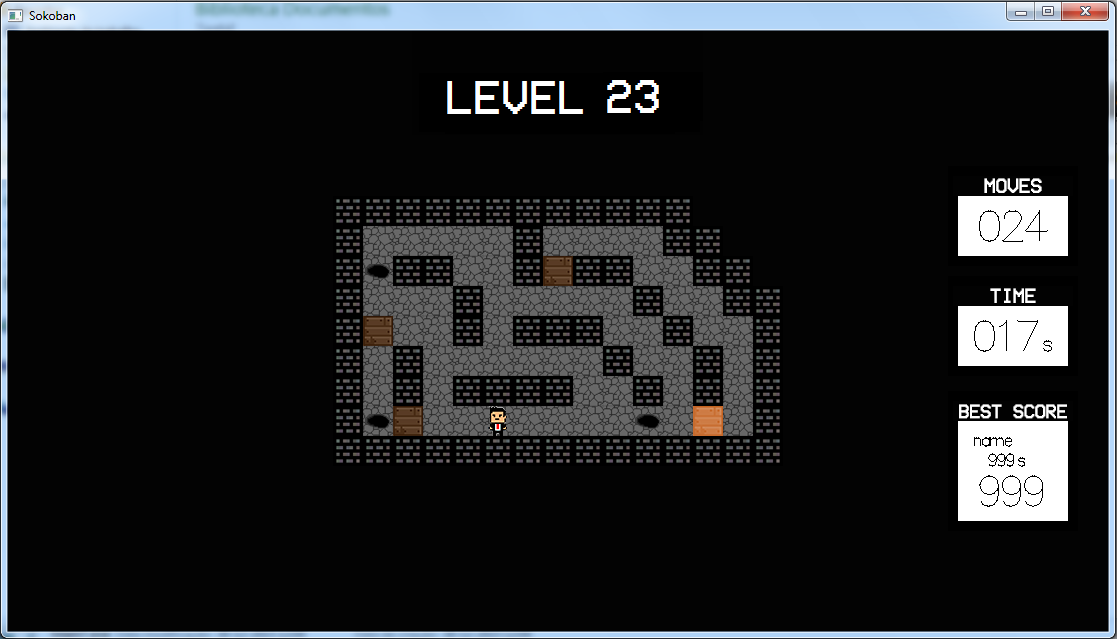
\includegraphics[width=8cm]{jogo.png}
\caption{Jogo a correr}
\end{figure}

\subsection{Extras}

Com o mínimo feito, decidimos adicionar alguns extras ao puzzle para melhor o programa final.

\begin{itemize}
\item \emph{Undo} (Tab) e \restart{Restart (Enter)}

Estas são, talvez, as duas funcionalidades adicionadas mais importantes. À semelhança do puzzle existente no sítio Sokoban.info, adicionámos a possibilidade de o jogador desfazer um movimento (\emph{Undo}) e de recomeçar o nível (\emph{Restart}). Antes disto, se o jogador se enganasse a clicar nas teclas, teria que fechar a aplicação e abri-la de novo. Dado que ao desfazer um movimento, o número de moves $x$ passa a $x-1$ (ver Figura~\ref{fig:undo}), o jogador pode usar esta funcionalidade para considerar um novo caminho, no qual efetue menos movimentos, e assim conseguir uma melhor pontuação. Para  tal, ao longo do jogo as posições do boneco e das caixas são guardadas e quando se retrocede uma jogada ou se recomeça  apenas se vai buscar ,respetivamente, a última ou a primeira lista das posições que estes ocuparam. 
\\
\\
\begin{figure}[H]
\centering
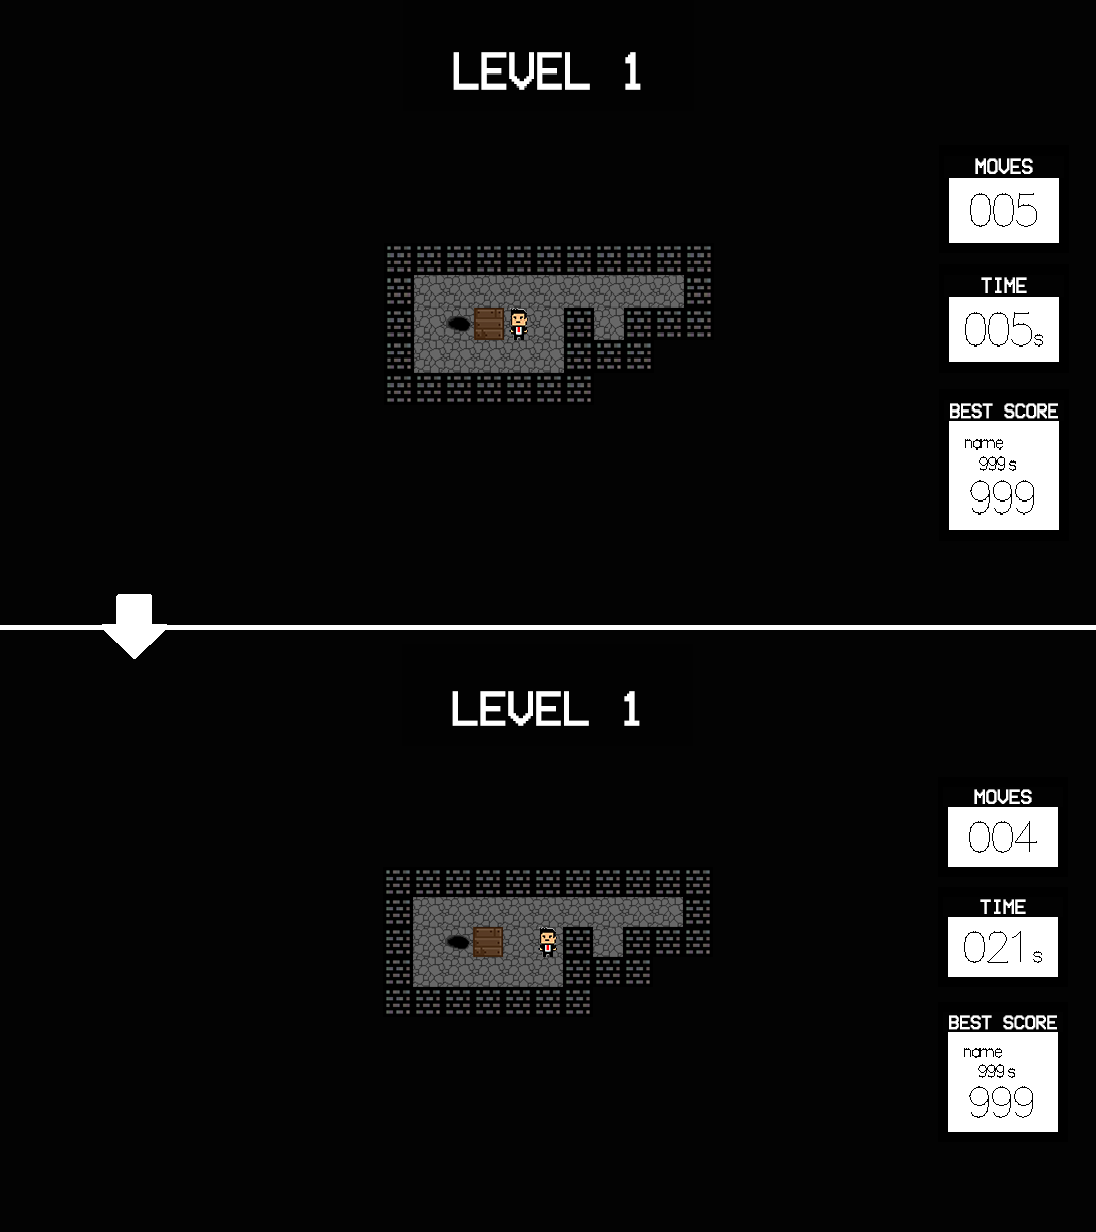
\includegraphics[width=8cm]{undo.png}
\caption{Jogo antes e depois de um \emph{undo}}
\label{fig:undo}
\end{figure}

\smallskip
\item Níveis

Sendo o \emph{Sokoban} um puzzle, pode ter vários mapas, com diferentes dificuldades. Assim, adicionámos diferentes níveis (30 ao todo) ao nosso, com diferentes dificuldades e diferentes números de caixas, sendo possível avançar e retroceder de nível.

Tanto avançar de nível (F2) como retroceder (F3) tem métodos muito similares. Como \emph{Mapa} dá-nos a informação do nível atual, ao pressionar F2 a função \texttt{nextlevel} carrega o nível seguinte, exceto no caso de se estar atualmente no nível 30 (último), ou o jogador ainda não ter carregado Enter para iniciar o jogo. Do mesmo modo a função \texttt{previouslevel} carrega o nível anterior, exceto se o jogador estiver no primeiro nível. Ambas as funções invocam a função \texttt{constroimapa} que, com a informação do nível, constrói um novo \emph{Mapa}.

\smallskip
\item \emph{Shuffle (F1)}

A funcionalidade de \emph{Shuffle} (Figura~\ref{fig:shuffle}) permite ao jogador, em cada nível, mudar a posição das caixas. Sendo que foi estipulado que o número máximo de \emph{shuffles} que um jogador pode fazer por nível é 3, isto implica que, para além da configuração inicial das caixas, o jogador pode tentar jogar o mesmo nível com outras três configurações. Para tal, ao carregar F1 o programa lê um ficheiro com as posições possíveis que as caixas podem ocupar - excluindo assim os lugares em que a finalização do nível seria impossível - e, através da função \texttt{randomRIO} escolhe aleatoriamente novos locais para as caixas, tendo em consideração aquelas que já estão num local de arrumação, ou seja, estas não são reposicionadas.

\begin{figure}[H]
\centering
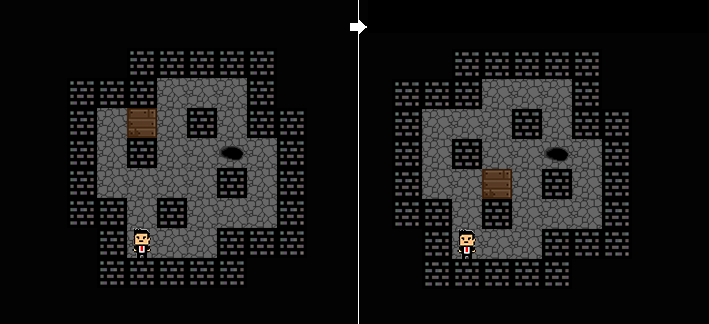
\includegraphics[width=12cm]{shuffle.png}
\caption{Jogo antes e depois de um \emph{shuffle}}
\label{fig:shuffle}
\end{figure}

\smallskip
\item \emph{Best Score}, nome e tempo

No \emph{Sokoban}, a \emph{score} corresponde, por padrão, ao número de movimentos efetuados por um jogador. Quanto menor for o número de movimentos, melhor é o score (i.e uma pessoa que completou um puzzle com 6 movimentos tem um melhor score que uma que usou 7 para o finalizar). Deste modo, assim que o jogador atingir uma pontuação melhor que a atual (antes de qualquer jogo a pontuação está em 999), o jogador pode associar o seu nome a ela. Se esse nível for jogado outra vez, essa pontuação vai ser mostrada, juntamente com o nome do jogador que a obteve, num retângulo com o nome de \emph{Best score} na interface do jogo, até que outro jogador, ou o mesmo, faça melhor.

Como é possível que o jogador faça o mesmo \emph{score} duas vezes, foi adicionado tempo à janela de jogo também. Quando o nível começa, o tempo começa a contar. O tempo servirá, portanto, como um ''desempate" no caso de o jogador obter a mesma \emph{score} duas vezes. Assim, se o número de movimentos for igual, a pontuação que conta como melhor, é aquela à qual está associada um menor tempo. 

Para facilitar foram criadas 3 funções : \texttt{concluido} que verifica se já terminou o nivel, \texttt{worse} e \texttt{best}, que verificam respestivamente se o desempenho foi pior ou melhor, do que aquele que obteu melhor pontuação.

{\footnotesize
\begin{Verbatim}
concluido m = equiv (coordenadas '.' (mapi m)) (tail (coord m))
worse m = (concluido m && (fst (score m)) == (snd (score m)) && fst (tempo m)>snd(tempo m))
                  || (concluido m && fst (score m)>snd (score m))
best m = (concluido m && fst (score m) == snd (score m) && fst (tempo m)<=snd (tempo m))
                 || (concluido m && fst (score m)<snd (score m))
\end{Verbatim}}

\end{itemize}

\subsection{Testes}

Para que tivéssemos a certeza de que as aplicações que nos foram pedidas estavam a funcionar bem e tinham o desempenho necessário, foram desenvolvidos testes para estas. Tanto para a função D como para a função E, usámos dois tipos de \emph{testing}: \emph{black-box} (tipo mooshak) e \emph{white-box} (HUnit).

Para os teste do tipo \emph{black-box}, tivemos que definir ficheiros de \emph{input} e \emph{output}. No ficheiro de \emph{output} púnhamos o \emph{output} esperado e ao testar, o programa iria comparar o \emph{output} do programa com o esperado. O \emph{white-box testing}, por sua vez, testa com conhecimento total do código. Como é possível testar funções individuais no código (testes unitários) e não apenas o \emph{input} e \emph{output} finais, proporciona uma maior cobertura do código.

Por exemplo, para a tarefa D, nos testes do tipo \emph{black-box}, tínhamos que criar um ficheiro .in com o mapa do jogo, seguido das coordenadas e da \emph{string} com os movimentos e um ficheiro .out com o resultado que esperávamos que o programa nos desse (\texttt{``INCOMPLETO <tick\_count>''} ou \texttt{``FIM <tick\_count>''}).

Quanto aos testes unitários, por exemplo na tarefa E, tínhamos uma lista de testes para a função principal, para podermos testar com todos os tipos de \emph{Pictures} do \emph{Gloss}. Um exemplo de um teste unitário para a Tarefa E é o seguinte:

\begin{Verbatim}

  t1 = TestCase (assertEqual "t1" "40 40" (tarefa5 (Circle 20))

\end{Verbatim}

Depois dos testes todos definidos, era só correr a função \texttt{main} dos testes no terminal que nos era dito a quantos testes o nosso código tinha passado (Figura \ref{fig:figuratestes}).

\begin{figure}[H]
\centering
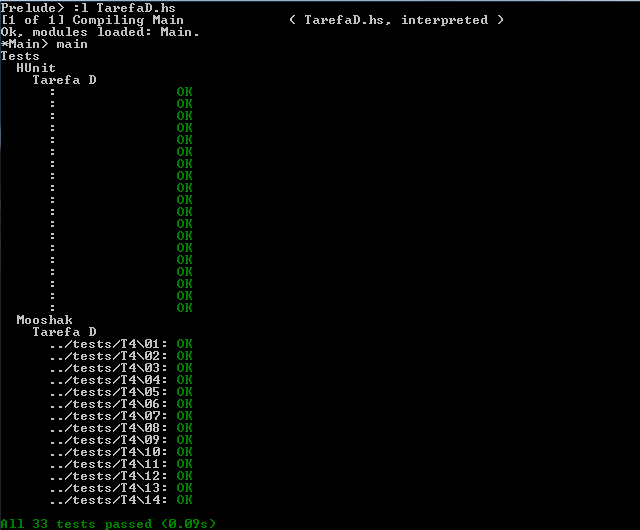
\includegraphics[width=8cm]{teste.png}
\caption{Indicação de que os testes foram todos passados no terminal}
\label{fig:figuratestes}
\end{figure}

\section{Conclusões}
\label{sec:conclusao}

Neste projeto, pretendíamos resolver as três tarefas que nos foram propostas, nomeadamente uma na qual tínhamos que criar a interface gráfica do jogo \emph{Sokoban}, e tornar possível a interação com este, associando comandos a teclas específicas (semelhante ao disponível em \href{sokoban.info}
{sokoban.info}).

Nas outras duas tarefas, pode-se dizer que atingimos os nossos objetivos, já que a plataforma pela qual somos avaliados (\emph{Mooshak}) aceitou a nossas resoluções.

Por sua vez, a última tarefa era aberta. Pretendíamos, para além do básico, adicionar alguns extras ao jogo, e conseguimos com que fosse possível ao jogador desfazer as últimas jogadas (\emph{undo}), recomeçar o jogo (\emph{restart}), ver quantas jogadas já fez no ecrã (número de \emph{moves}), e guardar a sua melhor \emoh{score} e associar o seu nome a esta. Para além disso, conseguimos com que o nosso jogo dispusesse de vários níveis com várias dificuldades, para poder dar uma melhor experiência de jogo a quem o jogar. Como atingimos todos os nossos objetivos, achámos que o resultado final foi muito positivo.

\end{document}